\documentclass{cheat-sheet}

\pdfinfo{
  /Title (Zusammenfassung Markovketten)
  /Author (Tim Baumann)
}

\usepackage{bbm} % Für 1 mit Doppelstrich (Indikatorfunktion)
\usepackage{mathtools} % psmallmatrix environment
\usepackage{nicefrac}

\usepackage{tikz}
\usetikzlibrary{matrix}

% Kleinere Klammern
\delimiterfactor=701

% TODO: Include-File für Stochastik

\renewcommand{\P}{\mathbb{P}} % Wahrscheinlichkeitsmaß
\newcommand{\E}{\mathbb{E}} % Erwartungswert
\newcommand{\ind}{\mathbbm{1}} % Indikatorfunktion
\newcommand{\iid}{i.\,i.\,d.} % identisch unabhängig verteilt
\DeclareMathOperator{\ggT}{ggT} % größter gemeinsamer Teiler
\newcommand{\Bor}{\mathfrak{B}} % Borel
\newcommand{\Alg}{\mathcal{A}} % Bezeichner für eine Sigma-Algebra
\newcommand{\Filt}{\mathcal{F}} % Filtration (von Sigma-Algebren)

\DeclareMathOperator{\var}{Var} % Varianz
\DeclareMathOperator{\cov}{Cov} % Kovarianz
\DeclareMathOperator{\cor}{Cor} % Korrelation

\DeclareMathOperator{\Beta}{Beta} % Beta-Verteilung

\definecolor{DefinitionColor}{rgb}{0.7,0.2,0.0}
\newcommand{\Defn}[1]{\textcolor{DefinitionColor}{#1}}

\begin{document}

\raggedcolumns % stretche Inhalt nicht über die gesamte Spaltenhöhe

\maketitle{Zusammenfassung Markovketten}

% Kapitel I. Endliche Markovketten
\section{Endliche Markovketten}

\begin{setting}
  Sei $E \neq \emptyset$ eine höchstens abzählbare Menge, die \textit{Zustandsmenge}.
  Eine \emph{stochastische Matrix}~$\Pi$ auf~$E$ ist geg. durch eine Abbildung $p : E \times E \to \cinterval{0}{1}$ mit
  \[
    {\sum}_{y \in E} p(x, y) = 1 \quad
    \forall\,x \in E.
  \]
\end{setting}

\begin{defn}
  Für einen \textit{Vektor} $\pi : E \to \R$ ist $\pi \Pi : E \to \R$ definiert durch
  \[
    (\pi \Pi)(x) \coloneqq {\sum}_{z \in E} \pi(z) \cdot p(z, x).
  \]
  (Annahme dabei: ${\sum}_{z \in E} \abs{\pi(z)} \cdot p(z, x) < \infty$ für alle $x \in E$.)
\end{defn}

% 1.1
\begin{defn}
  Eine Folge von ZVen $\{ X_n \in E \}$ heißt \emph{Markovkette} \textit{auf~$E$} mit \textit{Übergangsmatrix}~$p$, falls für alle $n \geq 1$ und $x_0, \ldots, x_{n+1} \in E$ gilt:
  \[
    \begin{array}{r l}
      & \P(X_{n+1} = x_{n+1} \,|\, X_0=x_0, \ldots, X_n=x_n) \\
      = & \P(X_{n+1} = x_{n+1} \,|\, X_n=x_n)
      = p(x_{n+1}, x_n)
    \end{array}
  \]
\end{defn}

\begin{interp}
  Bei gegebener Gegenwart $X_n = x_n$ ist die Zukunft $X_{n+1}$ unabhängig von der Vergangenheit.
\end{interp}

% 1.2
\begin{bem}
  Die Verteilung der ganzen Folge $\{ X_n \}$ ist durch die Verteilung von $X_0$ (\textit{Startverteilung}) und durch $p$ eindeutig bestimmt:
  \[
    \P(X_0=x_0, \ldots, X_n=x_n) = \P(X_0=x_0) \cdot {\prod}_{k=1}^n p(x_{n-1}, x_n)
  \]
  Gibt $\pi_0 : E \to \cinterval{0}{1}$ die Startverteilung an, und $\pi_n$ die Verteilung nach dem $n$-ten Schritt für $n \geq 1$, so gilt:
  \[
    \pi_n = \Pi^n \pi_0
  \]
\end{bem}

\begin{defn}
  Für $n \in \N$ und $x, y \in E$ ist
  \[
    \Defn{p^{(n)}(x, y)} \coloneqq \P(X_n=y \,|\, X_0=x)
  \]
  die \emph{$n$-Schritt-Übergangswahrscheinlichkeit} von~$x$ nach~$y$.
\end{defn}

\begin{lem}[\emph{Kolmogorov-Chapman-Gleichung}]
  Für $\ell, k \in \N$, $x, y \in E$ gilt
  \[
    p^{(k + \ell)}(x, y) = {\sum}_{z \in E} p^{(k)}(x, z) p^{(\ell)}(z, y).
  \]
\end{lem}

\begin{bem}
  Bekannte Spezialfälle:
  \[
    \begin{array}{r l}
      \text{\textit{Vorwärtsgleichung:}} & p^{(k+1)}(x, y) = {\sum}_{z \in E} \, p^{(k)}(x, z) p(z, y) \\
      \text{\textit{Rückwärtsgleichung:}} & p^{(k+1)}(x, y) = {\sum}_{z \in E} \, p(x, z) p^{(k)}(z, y)
    \end{array}
  \]
\end{bem}

% ausgelassen: Beispiel 1.3, 1.4, 1.5, 1.6

% Vorlesung vom 27.4.2017

% §2. Ergodensätze für endliche Markovketten

% 1.9
\begin{defn}
  Eine Verteilung $\pi$ heißt \emph{stationär}, falls $\pi = \pi \Pi$.
\end{defn}

% 1.7 + 1.8 + 1.10
\begin{satz}
  Sei $\{ X_n \}$ eine Markovkette auf einem endlichen Zustandsraum~$E$ mit der Übergangsmatrix~$\Pi$.
  Dann sind äquivalent:
  \begin{itemize}
    \item Es gibt ein $n_0 \geq 1$ mit $\fa{x, y \in E} p^{(n_0)}(x, y) > 0$.
    \item Es existiert ein $\pi : E \to \ocinterval{0}{1}$ mit
    \[
      p^{(n)}(x, y) \xrightarrow{n \to \infty} \pi(y)
      \quad \forall \, x, y \in E.
    \]
  \end{itemize}
  In diesem Fall ist $\pi$ die einzige stationäre Verteilung. \\
  Die Konvergenz ist exponentiell schnell:
  \[
    \abs{p^{(n)}(x, y) - \pi(y)} \leq C e^{- a n} \quad
    \text{für Konstanten $C, a > 0$.}
  \]
  Desweiteren gilt unabhängig von der Startverteilung
  \[
    \P(X_n = y) \xrightarrow{n \to \infty} \pi(y) \quad
    \forall \, y \in E.
  \]
\end{satz}

\begin{acht}
  Stationäre Verteil. können ohne Konvergenz existieren!
\end{acht}

% 1.11
\begin{satz}
  Falls $\fa{x, y \in E} p^{(n_0)}(x, y) > 0$ für ein $n_0 \in \N$, so gilt
  \[
    \tfrac{1}{n+1} \cdot {\sum}_{k=0}^n \ind \{ X_k = x \} \xrightarrow[n \to \infty]{\P} \pi(x)
    \quad \forall \, x \in E.
  \]
\end{satz}

% 1.12 (teilweise)
\begin{bem}
  Eine Übergangsmatrix heißt \emph{doppelt stochastisch}, falls
  \[
    {\sum}_{y \in E} p(x, y) = 1 \enspace \forall \, y \in E
    \quad \text{und} \quad
    {\sum}_{x \in E} p(x, y) = 1 \enspace \forall \, x \in E.
  \]
  Für jede solche Übergangsmatrix auf einem endlichen Raum ist die uniforme Verteilung stationär.
\end{bem}

% §. Paradoxon von Parrondo

\begin{bem}[\emph{Paradox von Parrondo}]
  Es gibt zwei Glücksspiele, bei denen man fast-sicher irgendwann all sein Geld verliert, dies aber nicht der Fall ist, falls man sie abwechselnd spielt!
  Diese Glücksspiele kann man als Markovketten modellieren, wobei der aktuelle Zustand durch die Anzahl an Euros im Besitz des Spielers gegeben ist.
\end{bem}

% Vorlesung vom 4.5.2017

% Kapitel II. Abzählbare Markovketten
\section{Abzählbare Markovketten}

% §2.1. Rekurrenz und Transienz

\begin{nota}
  Sei im Folgenden $\{ Z_n \}$ eine Markovkette auf einem abzählbaren Zustandsraum~$E$.
\end{nota}

% 2.1
\begin{defn}
  Für $x \in E$ und $n \in \N$ definiere die ZV \Defn{$\tau_x^{(n)}$} induktiv durch
  \[ \begin{array}{r c l}
    \tau_x^{(1)} &\coloneqq& \inf\,\Set{n > 0}{Z_n = x} \in \N \cup \{ \infty \} \\
    \tau_x^{(k)} &\coloneqq& \inf\,\Set{n > \tau_x^{(k-1)}}{Z_n = x}, \enspace k > 1.
  \end{array} \]
  (Beachte: $\tau_x^{(k)}$ ist eine messbare Abbildung.)
\end{defn}

\begin{bem}
  Ferner gilt $\{ \tau_x^{(k)} = n \} \in \sigma(Z_0, Z_1, \ldots, Z_n)$.
\end{bem}

\begin{defn}
  Für $x, y \in E$ sei
  $\Defn{F(x, y)} \coloneqq P(\tau_y^{(1)} < \infty \mid Z_0 = x)$
\end{defn}

% 2.2
\begin{lem}
  Für alle $x, y \in E$ und $k \geq 1$ gilt
  \[ P(\tau_y^{(k)} < \infty \mid Z_0 = x) = F(x, y) \cdot F(y, y)^{k-1}. \]
\end{lem}

\begin{bem}
  Setze $\Defn{\widetilde{\ell}(y)} \coloneqq {\sum}_{k=j}^\infty \ind \{ Z_k = y \}$.
  Dann gilt
  \[ P(\tau_y^{(k)} < \infty \mid Z_0 = x) = P(\widetilde{\ell} \geq k \mid Z_0 = x). \]
\end{bem}

% 2.3
\begin{defn}
  Ein Zustand $x \in E$ heißt
  \begin{itemize}
    \item \emph{absorbierend}, falls $p(x, x) = 1$,
    \item \emph{rekurrent}, falls $F(x, x) = 1$ und
    \item \emph{transient}, falls $F(x, x) < 1$.
  \end{itemize}
\end{defn}

\begin{bem}
  Absorbierende Zustände sind rekurrent.
\end{bem}

% ausgelassenes  Beispiel: a+1 Zustände nebeneinander, der linke und rechte sind absorbierend, die dazwischen haben eine Übergangswahrscheinlichkeit von 1/2 nach links und 1/2 nach rechts

% ausgelassenes Beispiel: Irrfahrt auf \N
% Falls $p \leq \nicefrac{1}{2}$, so ist Anfangszustand rekurrent
% Falls $p > \nicefrac{1}{2}$, so ist Anfangszustand transient
% Parondo-Paradoxon

\begin{bsp}
  In der Markovkette
  \begin{center}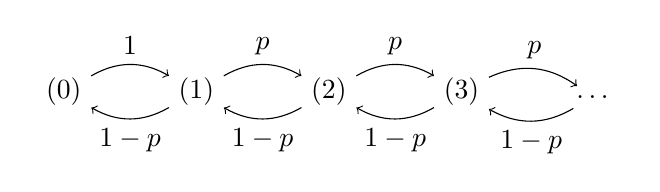
\begin{tikzpicture}
    \matrix [matrix of nodes, column sep=1cm, row sep=0.8cm] {
      \node (N0) {(0)}; &
      \node (N1) {(1)}; &
      \node (N2) {(2)}; &
      \node (N3) {(3)}; &
      \node (N4) {\ldots}; \\
    };
    \draw[->, bend left=30] (N0) to node [above] {$1$} (N1);
    \draw[->, bend left=30] (N1) to node [below] {$1 - p$} (N0);
    \draw[->, bend left=30] (N1) to node [above] {$p$} (N2);
    \draw[->, bend left=30] (N2) to node [below] {$1 - p$} (N1);
    \draw[->, bend left=30] (N2) to node [above] {$p$} (N3);
    \draw[->, bend left=30] (N3) to node [below] {$1 - p$} (N2);
    \draw[->, bend left=30] (N3) to node [above] {$p$} (N4);
    \draw[->, bend left=30] (N4) to node [below] {$1 - p$} (N3);
  \end{tikzpicture}\end{center}
  ist (0) genau dann rekurrent, falls $p \leq \nicefrac{1}{2}$, ansonsten transient.
  \TODO{genauer!}
\end{bsp}

% 2.6
\begin{defn}
  Die \emph{Anzahl der Besuche} in~$y \in E$ ist
  \[
    \Defn{\ell(y)} \coloneqq {\sum}_{k=0}^\infty \ind \{ Z_k = y \}.
  \]
  Die \emph{Green'sche Funktion} von $\{ Z_n \}$ ist $G : E \times E \to \cinterval{0}{\infty}$ mit
  \[
    \Defn{G(x, y)} \coloneqq \E(\ell(y) \mid Z_0 = x).
  \]
\end{defn}

\begin{bem}
  $
    \begin{array}[t]{r c l}
      G(x, y) &=& \E \left( {\sum}_{k=0}^\infty \ind \{ Z_k = y \} \mid Z_0 = x \right) \\
      &=& {\sum}_{k=0}^\infty P(Z_k = y \mid Z_0 = x) \\
      &=& \delta_{xy} + {\sum}_{k=1}^\infty p^{(k)}(x, y).
    \end{array}
  $
\end{bem}

% 2.7
\begin{satz}
  Für alle $x, y \in E$ gilt
  \[
    G(x, y) =
    \begin{cases}
      F(x, y)/(1 - F(y, y)) & \text{falls $x \neq y$}, \\
      1/(1 - F(y, y)) & \text{falls $x = y$}. \\
    \end{cases}
  \]
\end{satz}

\begin{kor}
  $x$ ist rekurrent $\iff$ $G(x, x) = \infty$
\end{kor}

\begin{lem}
  Ist $F(x, y) \in \ointerval{0}{1}$, so ist $x$ nicht rekurrent.
\end{lem}

% 2.8
\begin{satz}
  Ist $x \in E$ rekurrent und $F(x, y) > 0$, so ist $y$ auch rekurrent und $F(x, y) = F(y, x) = 1$.
\end{satz}

% nicht in der Vorlesung
\begin{satz}
  Es sind äquivalent:
  \begin{itemize}
    \miniitem{0.9 \linewidth}{$x$ ist rekurrent}
    \miniitem{0.3 \linewidth}{$F(x, x) = 1$}
    \miniitem{0.5 \linewidth}{$\fa{y \in E} F(x, y) \in \{ 0, 1 \}$}
    \miniitem{0.3 \linewidth}{$G(x, x) = \infty$}
    \miniitem{0.5 \linewidth}{$\fa{y \in E} G(x, y) \in \{ 0, \infty \}$}
  \end{itemize}
\end{satz}

\iffalse
% 2.9
\begin{interp}
  %Die Aussage kann man wie folgt deuten:
  $F(x, y) > 0$ bedeutet, dass nach jedem Besuch in~$x$ der Zustand $y$ auch besucht wird mit positiver Wahrscheinlichkeit und die Rekurrenz von~$x$ bedeutet, dass $x$ unendlich oft besucht wird.
  Der Satz sagt, dass dann auch $y$ unendlich oft besucht wird.
\end{interp}
\fi

% 2.9
\begin{bem}
  $F(x, y) > 0 \iff \ex{n \geq 1} p^{(n)}(x, y) > 0$
\end{bem}

% 2.10
\begin{defn}
  $\{ Z_n \}$ heißt \emph{irreduzibel}, falls $\fa{x, y \in E} F(x, y) > 0$.
\end{defn}

% 2.11
\begin{satz}
  Sei $\{ Z_n \}$ irreduzibel.
  Dann sind entweder alle Zustände rekurrent oder alle Zustände transient.
\end{satz}

% Vorlesung vom 9.5.2017

% 2.12
\begin{satz}
  Irreduzible Ketten auf endlichen Räumen sind rekurrent.
\end{satz}

% §2. Rekurrenz und Transienz von Irrfahrten
\section{Rekurrenz und Transienz von Irrfahrten}

\begin{situation}
  $\{ Z_n \}$ ist eine Irrfahrt auf $\Z^d$, \dh{}
  \[ p(x, y) = p(0, y - x) =: q(y - x). \]
  Mit and. Worten: Die \textit{Zuwächse} $\{ Z_n - Z_{n-1} \}_{n \geq 1}$ sind \iid{} ZVn.
\end{situation}

\begin{bsp}
  Einfache Irrfahrt auf~$\Z$: \quad
  $p(0, 1) = p$, $p(0, -1) = q = 1 - p$
\end{bsp}

%Für welche Werte von $p$ ist diese Irrfahrt rekurrent/transient?

In diesem Fall kann man die Greensche Funktion exakt berechnen:

\[
  \begin{array}{r c l}
    G(x, x) &=& G(0,0) \\
    &=& {\sum}_{m=0}^\infty p^{(m)}(0, 0) \\
    &=& 1 + {\sum}_{n=1}^\infty p^{(2n)}(0, 0) \\
    &=& 1 + {\sum}_{n=1}^\infty \tbinom{2n}{n} p^n (1-p)^n \\
    &=& 1 + {\sum}_{n=1}^\infty \tbinom{2n}{n} 4^{-n} (4 p (1-p))^n \\
    &=& (1 - 4 p (1-p))^{-1/2} \\
    &=& 1/\abs{2p - 1}
  \end{array}
\]

% 2.13
\begin{satz}
  Sei $\{ Z_n \}$ eine Irrfahrt auf~$\Z$ mit
  \[ \E \abs{Z_1 - Z_0} = {\sum}_{x \in \Z} \abs{x} p(0, x) < \infty. \]
  Dann gilt: \quad
  $
    \{ Z_n \} \text{ ist rekurrent} \iff {\sum}_{x \in \Z} \, x p(0, x) = 0.
  $
\end{satz}

\begin{defn}
  Die \emph{einfache symmetrische Irrfahrt auf $\Z^d$} ist die translationsinvariante Markovkette mit
  \[
    p(0, \pm e_i) = \tfrac{1}{2 d} \quad \text{für } i = 1, \ldots, d.
  \]
\end{defn}

\begin{bem}
  Für einfache symmetrische Irrfahrten gilt:
  \[
    p^{(2n)}(x, x) = \qquad \sum_{\mathclap{\substack{k_1, \ldots, k_d \in \N \\ k_1 + \ldots + k_d = n}}} \qquad \frac{(2n)!}{(k_1!)^2 \cdots (k_d!)^2} (\frac{1}{2d})^{2n}
  \]

  Für $d = 2$ gilt $p^{(2n)}(0, 0) = \left[ \tbinom{2n}{n} (\tfrac{1}{2})^{2n} \right]^2$.
  Mit der Stirling'schen Formel folgt $p^{(2n)}(0, 0) \approx \tfrac{1}{\pi n}$.
  Somit gilt $\sum p^{(2n)}(0,0) = \infty$.
\end{bem}

\begin{fazit}
  Die zweidimensionale einfache symm. Irrfahrt ist rekurrent.
\end{fazit}

% Vorlesung vom 11.5.2017

\begin{bem}
  Man kann zeigen:
  Für einfache symm. Irrfahrten auf~$\Z^d$ gilt
  \[ p^{(2n)}(0,0) \leq C_d / n^{\nicefrac{d}{2}} \]
  für eine Konstante $C_d > 0$.
  Somit ist die einfache Irrfahrt transient für alle $d \geq 3$.
\end{bem}

\begin{defn}
  $\Defn{\varphi(t)} \coloneqq {\sum}_{x \in \Z^d} e^{i (t \cdot x)} p(0, x)$ \quad
  für $t \in \R^d$
\end{defn}

\begin{bem}
  Da die Zuwächse $\{ Z_n - Z_{n-1} \}$ \iid{} sind, gilt
  \[ {\sum}_{x \in \Z^d} \, e^{i (t \cdot x)} p^{(n)}(0, x) = \varphi^n(t), \quad n \geq 1 \]

  \textit{Inversionsformel}: \quad
  $p^{(n)}(0, x) = \tfrac{1}{(2 \pi)^d} \Int{\cointerval{-\pi}{\pi}^d}{}{e^{- i (t \cdot x)} \varphi^n(t)}{t}$
\end{bem}

\begin{satz}
  Für jede Irrfahrt $\{ Z_n \}$ auf $\Z^d$ gilt
  \[ G(0, 0) = \left( \frac{1}{2 \pi} \right)^d \lim_{\lambda \uparrow 1} \Int{t \in \cointerval{-\pi}{\pi}^d}{}{Re(\tfrac{1}{1 - \lambda \varphi(t)})}{t} = \infty \]
\end{satz}

\begin{bsp}
  Für die einfache symm. Irrfahrt $\{ Z_n \}$ auf~$\Z^d$ ist
  \[
    \varphi(t) = \tfrac{1}{d} {\sum}_{k=1}^d \cos(t_k)
  \]
  Mit der Ungleichung $1 - \cos(u) \geq c_0 u^2$ für alle $u \in \cinterval{- \pi}{\pi}$ folgt
  \[
    \varphi(t) \geq \tfrac{c_0}{d} \abs{t}^2.
  \]
  Es folgt
  \[
    \tfrac{1}{1 - \lambda \varphi(t)} \leq \tfrac{d}{\lambda c_0} \abs{t}^{-2}
  \]
  Die Funktion $\abs{t}^{-2}$ ist auf $\cointerval{-\pi}{\pi}^d$ für jedes $d \geq 3$ integrierbar.
  Somit ist die einfache Irrfahrt auf $\Z^d$, $d \geq 3$, transient.
\end{bsp}

% 2.16
\begin{satz}
  Jede irreduzible Irrfahrt auf $\Z^d$ mit $d \geq 3$ ist transient.
\end{satz}

% 2.17
\begin{bsp}
  Sei $\{ Z_n \}$ eine Irrfahrt auf $\Z$ mit $p(0, x) = p(0, -x)$.
  Gelte
  \[ x^\alpha p(0, x) \xrightarrow{x \to \infty} c \in \ointerval{0}{\infty} \]
  für ein $\alpha > 1$.
  Dann ist
  \[
    1 - \varphi(t) = \sum_{\mathclap{n=-\infty}}^\infty (1{-}\cos(nt)) p(0, n)
    \enspace \text{und} \enspace
    \frac{1 {-} \varphi(t)}{\abs{t}^{\alpha - 1}} = \sum_{\mathclap{n=-\infty}}^\infty \abs{n}^\alpha p(0, n) \abs{t} f(n t)
  \]
  mit $f(x) = (1 - \cos(x))/\abs{x}^\alpha$.
  Außerdem $\abs{n}^\alpha p(0, n) = c + \epsilon_n$, wobei $\epsilon_n \to 0$ für $\abs{n} \to \infty$.
  Es folgt
  \[
    \tfrac{1 - \varphi(t)}{\abs{t}^{\alpha - 1}} = \sum_{n=-\infty}^\infty c \abs{t} f(n t) + \sum_{n=-\infty}^\infty \epsilon_n \abs{t} f(n t).
  \]
  Für $t \to 0$ hat man
  \[
    \sum_{n=-\infty}^\infty \abs{t} f(n t) \to \Int{-\infty}{\infty}{f(x)}{x}
    \enspace \text{und} \enspace
    \sum_{n=-\infty}^\infty \epsilon_n \abs{t} f(n t) \to 0.
  \]
  Es folgt für $\alpha < 3$:
  \[ \lim_{t \to 0} \tfrac{1 - \varphi(t)}{\abs{t}^{\alpha - 1}} = c \Int{-\infty}{\infty}{\tfrac{1 - \cos(x)}{\abs{x}^\alpha}}{x} < \infty \]
  Folglich ist $\tfrac{1}{1 - \varphi(t)}$ für $\alpha < 2$ integrierbar und somit $\{ Z_n \}$ transient.

  Für $\alpha = 2$ ist $1/(1 - \varphi(t))$ in der Umgebung von null nicht integrierbar und damit $\{ Z_n \}$ rekurrent.

  Für $\alpha > 2$ ist $\sum \abs{x} p(0, x) < \infty$ und somit ist die Irrfahrt rekurrent, da der Erwartungswert der Zuwächse null ist.
\end{bsp}

% Vorlesung vom 16. Mai 2017

% §3. Erneuerungstheorie
\section{Erneuerungstheorie}

\begin{situation}
  Seien $\{ X_k \}_{k \geq 1}$ unabhängige ZVn mit Werten in~$\N$ und $P(X_k \geq 1) > 0$, wobei $\{ X_k \}_{k \geq 2}$ identisch vert. sind.
  Dann definiert
  \[
  Z_n \coloneqq {\sum}_{k=1}^n X_k + Z_0
  \]
  eine Irrfahrt $\{ Z_n \}_{n \geq 0}$ mit nicht-negativen Zuwächsen auf~$\Z$.
\end{situation}

\begin{ziel}
  Untersuche das asympt. Verhalten von $G(0, x)$.
\end{ziel}

\begin{defn}
  Die \emph{erzeugende Funktion} einer Folge $\{ a_n \}$ ist
  \[ A(s) \coloneqq {\sum}_{n=0}^\infty a_n s^n. \]
\end{defn}

% 2.18
\begin{bsp}
  Setze $p_k \coloneqq P(X_2 = k)$, $k \geq 0$.
  Wir nehmen an, dass
  \[ a \coloneqq \E[X_2] = {\sum}_{k=1}^\infty k p_k \in \ointerval{0}{\infty}. \]
  Definiere
  $q_k \coloneqq \tfrac{1}{a} {\sum}_{j=k}^\infty p_j$
  für $k \geq 1$.
  Dann ist ${\sum}_{k=1}^\infty q_k = 1$. \\
  Sei $X_1$ eine ZV mit $P(X_1=k) = q_k$, $k \geq 1$.
  Setze
  \[
    \begin{array}{r c l}
      f(s) &\coloneqq& {\sum}_{k=1}^\infty p_k s^k = \E[s^{X_2}], \enspace \abs{s} \leq 1 \\[0.1cm]
      g(s) &\coloneqq& {\sum}_{k=1}^\infty q_k s^k = \E[s^{X_1}] \\[0.1cm]
      \psi(s) &\coloneqq& {\sum}_{x=1}^\infty G(0, x) s^x, \enspace \abs{s} < 1
    \end{array}
  \]
  Dann gilt für $\abs{s} < 1$:
  \[ \psi(s) = {\sum}_{k=1}^\infty g(s) f(s)^{k-1} = g(s)/(1 - f(s)) \]
  Außerdem gilt:
  \[ g(s) = \tfrac{s}{a (1-s)} (1 - f(s)) \]
  Es folgt:
  \[ \psi(s) = \sum_{x=1}^\infty \tfrac{1}{a} s^x \]
  Somit ist $G(0, x) = \tfrac{1}{a}$.
\end{bsp}

% 2.19
\begin{satz}
  Angenommen, $\ggT \Set{k}{p_k > 0} = 1$.
  Dann gilt für jede Verteilung von~$X_1$, dass
  \[ G(0, x) \xrightarrow{x \to \infty} \tfrac{1}{a}. \]
\end{satz}

% 2.20
\begin{lem}
  Sei $g(\theta)$ integrierbar auf $\cointerval{-\pi}{\pi}$.
  Dann gilt
  \[
    \Int{\cointerval{-\pi}{\pi}}{}{e^{i \theta x} g(\theta)}{\theta} \xrightarrow{\abs{x} \to \infty}
    \quad (x \in \Z)
  \]
\end{lem}

% 2.21
\begin{lem}
  \begin{minipage}[t]{0.8 \linewidth}
    Seien alle $X_k$ identisch verteilt und $\ggT \Set{p}{p_k > 0} = 1$.
    Dann existiert $L \coloneqq {\lim}_{x \to \infty} G(0, x)$.
  \end{minipage}
\end{lem}

% 2.22
\begin{defn}
  Seien $\{ X_k \}_{k \geq 1}$ unabhängige, nichtneg. ZVn und seien $\{ X_k \}_{k \geq 2}$ identisch verteilt.
  Setze $Z_n \coloneqq {\sum}_{k=1}^n X_k$.
  Dann heißt
  \[
    \begin{array}{r c l l}
      \Defn{\eta(t)} &\coloneqq& \min\,\Set{k \geq 1}{Z_k > t} &
      \text{\emph{Erneuerungsprozess} und} \\
      \Defn{H(t)} &\coloneqq& \E[\eta(t)]
      & \text{\emph{Erneuerungsfunktion}.}
    \end{array}
  \]
\end{defn}

Falls $X_k$ nur Werte aus~$\N$ annimmt, so können wir das Verhalten von $H(t) - H(t-1)$ wie folgt beschreiben:
\[\begin{array}{r l}
  & H(t) = \E[\eta(t)] = \sum_{k=0}^\infty P(\eta(t) > k) = \sum_{k=0}^\infty P(Z_k \leq t) \\
  \rightsquigarrow & H(t) - H(t-1) = \sum_{k=0}^\infty P(Z_k = t) \xrightarrow{t \to \infty} 1/\E[X_2].
\end{array}\]

\begin{defn}
  $
    \begin{array}[t]{r c l l}
    \Defn{\gamma(t)} &\coloneqq& t - Z_{\eta(t)-1} \geq 0 & \text{heißt \emph{Undershoot},} \\
    \Defn{\chi(t)} &\coloneqq& Z_{\eta(t)} - t > 0 & \text{heißt \emph{Overshoot}.}
    \end{array}
  $
\end{defn}

\begin{satz}
  Sind die Bedingungen des letzten Satzes erfüllt, so gilt
  \[
    P(\gamma(t)=i, \chi(t)=j) \xrightarrow{t \to \infty} \frac{p_{i+j}}{\E[X_2]}
    \qquad \text{für alle } i \geq 0, j \geq 1.
  \]
\end{satz}

\begin{kor}
  $
    \begin{array}[t]{r c l}
      P(\gamma(t) = i) &\xrightarrow{t \to \infty}& \tfrac{1}{a} {\sum}_{k=i+1}^\infty p_k, \\[0.15cm]
      P(\gamma(t) = j) &\xrightarrow{t \to \infty}& \tfrac{1}{a} {\sum}_{k=j}^\infty p_k
    \end{array}
  $
\end{kor}

\TODO{Eine der Gleichungen im Korollar sollte $\chi$ beinhalten.}

% Vorlesung vom 23.5.2017

% §4. Positive Rekurrenz
\section{Positive Rekurrenz}

% 2.25
\begin{defn}
  $x \in E$ heißt \emph{positiv rekurrent}, falls $\E [\tau_x^{(1)} | Z_0=x] < \infty$. \\
  Ist $x$ rekurrent, aber nicht pos. rekurrent, so heißt $x$ \emph{nullrekurrent}.
\end{defn}

\begin{bem}
  positive Rekurrenz $\implies$ Rekurrenz
\end{bem}

% 2.26
\begin{lem}
  \begin{minipage}[t]{0.8 \linewidth}
    Sei $x$ ein positiv rekurrenter Zustand. \\
    Ist $F(x, y) > 0$, so ist auch~$y$ positiv rekurrent.
  \end{minipage}
\end{lem}

% 2.27
\begin{kor}
  Ist $\{ Z_n \}$ irreduzibel und $x_0 \in E$ positiv rekurrent, so gilt:
  \begin{itemize}
    \item alle Zustände sind positiv rekurrent
    \item $\Defn{m(x, y)} \coloneqq \E[ \tau^{(1)}_y | Z_0 = x ] < \infty$ für alle $x, y \in E$
  \end{itemize}
\end{kor}

% 2.28
\begin{defn}
  Die Zahl
  $d_x \coloneqq \ggT \Set{n \geq 1}{p^{(n)}(x,x) > 0}$
  heißt \emph{Periode} von~$x$.
  Falls $d = d_x$ für alle $x \in E$, so heißt $d$ \textit{Periode} der Kette~$\{ Z_n \}$.
\end{defn}

% 2.29
\begin{lem}
  Ist $\{ Z_n \}$ irreduzibel, so gilt $d_x = d_y$ für alle $x, y \in E$.
\end{lem}

% 2.30
\begin{satz}
  Es gibt eine Familie $\{ \pi_y \in \R_{> 0} \}_{y \in E}$, sodass
  \[ \fa{x, y \in E} p^{(n)}(x, y) \xrightarrow{n \to \infty} \pi_y \]
  genau dann, wenn
  \begin{itemize}
    \item $\{ Z_n \}$ irreduzibel und
    \item aperiodisch (\dh{} $d = 1$) ist und
    \item ein $x_0$ existiert, sodass $m(x_0, x_0) < \infty$.
  \end{itemize}
  Die Folge $\{ \pi_y \}_{y \in E}$ ist die eindeutige Lösung zu
  \[
    \left\{
      \begin{array}{l}
        {\sum}_{y \in E} \abs{P_y} < \infty \\
        {\sum}_{y \in E} \pi_y = 1 \\
        {\sum}_{x \in E} \pi_x p(x, y) = \pi_y \text{ für alle } y \in E
      \end{array}
    \right.
  \]
  Es gilt $\pi_y = 1/m(y,y)$.
\end{satz}

% Vorlesung vom 30.5.2017

% 2.31
\begin{defn}
  Eine Verteilung $\{ \mu_x \}_{x \in E}$ auf~$E$ heißt \emph{stationär}, falls
  \[
    \mu_x = {\sum}_{y \in E} \mu_y p(y, x)
    \quad \text{für alle $x \in E$}
    \qquad \text{(kurz: $\mu = \mu P$).}
  \]
\end{defn}

\begin{bem}
  Für eine stationäre Verteilung $\{ \mu_x \}_{x \in E}$ gilt
  \[
    \mu_x = {\sum}_{y \in E} \mu_y p^{(n)}(y, x)
    \quad \text{für alle $x \in E$ und $n \in \N$}
  \]
\end{bem}

% 2.33
\begin{lem}
  Sei $x$ ein positiv rekurrenter Zustand.
  Dann definiert
  \[
    \Defn{\mu_y^{(x)}} \coloneqq \frac{1}{m(x, x)} \cdot \E \left[ \sum_{k=0}^{\tau_x^{(1)} - 1} \ind \{ Z_k = y \} \middle| Z_0 = x \right]
  \]
  für alle $y \in E$ eine stationäre Verteilung $\{ \mu_y^{(x)} \}_{y \in E}$.
\end{lem}

% 2.34
\begin{satz}
  Sei $\{ Z_n \}$ eine irreduzible Kette.
  Dann gilt:
  \[
    \{ Z_n \} \text{ ist pos. rekurrent} \iff
    \{ Z_n \} \text{ hat eine stationäre Verteilung.}
  \]
  In diesem Fall ist die stationäre Verteilung eindeutig.
\end{satz}

% $\Defn{\sigma_x^n} \coloneqq \sup \Set{k \leq n}{Z_k = x} \in \{ - \infty, 0, \ldots, n \}$

% 2.35
\begin{satz}
  Eine irreduzible Kette auf einem endlichen Zustandsraum ist immer positiv rekurrent.
  Ferner existieren $C > 0$ und $q \in \ointerval{0}{1}$ mit
  \[
    P(\tau_y^{(1)} > n \,|\, Z_0 = x) < C q^n
    \quad \text{für alle $n \geq 1$ und $x, y \in E$.}
  \]
\end{satz}

% 2.36
\begin{satz}
  Sei $\{ Z_n \}$ irreduzibel und positiv rekurrent. \\
  Sei $f : E \to \R$ integrierbar bezüglich der stationären Verteilung $\{ \pi_x \}$, \dh{} ${\sum}_{x \in E} \abs{f(x)} \pi_x < \infty$.
  Dann gilt
  \[
    \tfrac{1}{n} \sum_{k=0}^{n-1} f(Z_k) \xrightarrow{\text{f.\,s.}} \sum_{x \in E} f(x) \pi_x
  \]
\end{satz}

\begin{bsp}
  Für $f(y) \coloneqq \ind \{ y = x_0 \}$ für eine $x_0 \in E$ erhalten wir
  \[ \tfrac{1}{n} \sum_{k=0}^{n-1} \ind \{ Z_k = x_0 \} \xrightarrow{\text{f.\,s.}} \pi_{x_0}. \]
  Es folgt mit majorisierter Konvergenz:
  \[ \tfrac{1}{n} \sum_{k=0}^{n-1} p^{(k)}(x, x_0) \xrightarrow{n \to \infty} \pi_{x_0}. \]
\end{bsp}

\begin{bsp}
  Sei $\{ Z_n \}$ irreduzibel, periodisch mit Periode $p > 1$.
  Dann gilt
  \[
    p^{(dk)}(x_0, x_0) \xrightarrow d / m(x_0, x_0).
  \]
\end{bsp}

% 2.37
\begin{lem}
  Sei $\{ Z_n \}$ eine irreduzible Kette mit der Periode $d \geq 1$. \\
  Für jedes $x \in E$ existiert ein $m_x \geq 1$ mit
  \[
    p^{(md)}(x, x) > 0
    \text{für alle $m \geq m_x$.}
  \]
\end{lem}

% Vorlesung vom 13. Juni 2017

% 2.38
\begin{prop}
  Sei $\{ Z_n \}$ irreduzibel und periodisch mit $d \geq 1$. \\
  Dann existieren paarweise disjunkte $C_0, C_1, \ldots, C_{d-1} \subseteq E$ mit $C_0 \cup \ldots \cup C_{d-1} = E$ und
  \[
    \Set{y \in E}{x \in C_i, p(x, y) > 0} = C_{(i+1) \% d}.
  \]
  In anderen Worten: Die Mengen $C_i$ werden zyklisch besucht.
\end{prop}

% 2.39
\begin{bem}
  Die Markovkette $\{ Z_{md} \}_{m \geq 0}$ ist nicht irreduzibel (für $d > 1$) aber die Restriktion auf jedes $C_i$ ist irreduzibel und außerdem aperiodisch.
  Mit dem Ergodensatz erhalten wir
  \[
    p^{(md)}(x, y) \xrightarrow{m \to \infty} d / m(y, y)
    \quad \text{für alle $x, y \in C_i$}
  \]
  Falls $x \in C_0$ und wir wollen $p^{(md + r)}(x, y)$ berechnen, so reicht es $y \in C_r$ zu betrachten.
  %, weil
  %\[
  %  p^{(md + r)}(x, y) = 0
  %  \quad \text{für alle $y \in E \setminus C_r$}
  %\]
  Definiere
  \[
    F_r(x, y) \coloneqq \P(\tau_y^{(1)} < \infty, \, \tau_y^{(1)} \equiv r \, (\mathrm{mod}\, d) \,|\, Z_0 = x)
  \]
  Es gilt dann:
  \[
    p^{(md+r)}(x, y) \xrightarrow{m \to \infty} F_r(x, y) d / m(y, y)
  \]
\end{bem}

%\begin{bsp}
%  Seien $\{ \xi_n \}$ \iid{} mit $P(\xi_1 = 1) = P(\xi_1 = 0) = 1/2$.
%  Setze $X_n \coloneqq {\sum}_{i=1}^n 2^{i-1} \xi_i$.
%  Dann gilt $X_n \xrightarrow{\omega} U_{\cinterval{0}{1}}$, wobei $U_{\cinterval{0}{1}}$ die uniforme Verteilung auf~$\cinterval{0}{1}$ ist.
%\end{bsp}

% §3. Martingale
\section{Martingale}

% §3.1. Definition und einfache Eigenschaften

Sei im Folgenden $(\Omega, \mathcal{F}, P)$ ein Maßraum.

% 3.1
\begin{defn}
  Eine wachsende Folge $\Filt_0 \subseteq \Filt_1 \subseteq \ldots$ von $\sigma$-Algebren heißt \emph{Filtration}.
  Eine Folge von ZVen $\{ M_n \}$ heißt \emph{adaptiert} an die Filtration $\{ \Filt_n \}$, falls $M_n$ $\Filt_n$-messbar ist für jedes $n \geq 0$.
\end{defn}

% 3.2
\begin{defn}
  Sei $X$ eine ZV mit $\E[\abs{X}] < \infty$.
  Dann heißt $\widehat{X}$ \emph{bedingte Erwartung} von~$X$ bzgl. $\sigma$-Algebra~$\mathcal{A}$ falls
  $\hat{X}$ $\mathcal{A}$-messbar ist und $\E[X \ind_A] = \E[\hat{X} \ind_A]$ für alle $A \in \mathcal{A}$.
\end{defn}

% 3.2
\begin{defn}
  Eine $\{ F_n \}$-adapt. Folge $\{ M_n \}$ mit $\fa{n\!}\! \E[\abs{M_n}] < \infty$ heißt
  \[
    \left. \begin{array}{l}
      \text{\emph{Martingal}}\\
      \text{\textit{Submartingal}}\\
      \text{\textit{Supermartingal}}\\
    \end{array} \right\}
    \enspace \text{falls} \enspace
    \E[M_{n+1} | \Filt_n]
    \left\{ \begin{array}{l}
      =\\
      \geq\\
      \leq
    \end{array} \right\}
    M_n
    \quad \forall\,n \geq 0.
  \]
\end{defn}

% 3.3
\begin{bem}
  \begin{itemize}
    \item $\{ M_n \}$ ist Submartingal $\iff$ $\{ -M_n \}$ ist Supermartingal
    \item $\{ M_n \}$ ist Martingal $\iff$ $\{ M_n \}$ ist Super- und Submartingal
  \end{itemize}
\end{bem}

\begin{bem}
  Martingal-Strategie für wdh. Werfen einer fairen Münze:
  \begin{itemize}
    \item 1. Runde: Einsatz = 1 Euro, bei Gewinn Ausstieg
    \item 2. Runde: Einsatz = 2 Euro, bei Gewinn Ausstieg, \ldots
    \item $n$. Runde: Einsatz = $2^{n-1}$ Euro, bei Gewinn Ausstieg
  \end{itemize}
  Es gilt: $T = \inf \Set{ n \geq 1 }{ \text{$n$-te Runde ist gewonnen} } < \infty$ fast sicher, der Gewinn ist $1$ Euro.
\end{bem}

\begin{bsp}
  Seien $\{ X_i \}$ unabh. ZVen mit $\E[X_i] = 0$ for alle $i \geq 0$.
  Sei $M_n \coloneqq X_1 + \ldots + X_n$.
  Dann ist $\{ M_n \}$ ein Martingal bzgl. der Filtration $\{ \Filt_n \}$ mit $\Filt_n \coloneqq \sigma(X_1, \ldots, X_n)$.
\end{bsp}

\begin{defn}
  Für eine Folge $\{ M_n \}$ von ZVen heißt $\{ \sigma(M_0, M_1, \ldots, M_n) \}_{n \geq 0}$ \emph{natürliche Filtration}.
\end{defn}

% 3.5
\begin{lem}
  Ist $\{ M_n \}$ ein Martingal bzgl. einer bel. Filtration, so ist $\{ M_n \}$ auch ein Martingal bzgl. der natürlichen Filtration.
\end{lem}

\begin{defn}
  $
    \arraycolsep=1pt
    \begin{array}[t]{r c l}
      \{ M_n \} \text{ ist Martingal} & \coloniff & \{ M_n \} \text{ ist Martingal bzgl.} \\
      && \text{der natürlichen Filtration}
    \end{array}
  $
\end{defn}

% 3.7
\begin{lem}
  Ist $\{ M_n \}$ ein Submartingal, so gilt $\E[ M_{i+1} ] \geq \E[M_i]$.
\end{lem}

% 3.8
\begin{lem}
  Sei $\{ M_n \}$ ein Martingal bzgl. $\{ \Filt_n \}$.
  Dann gilt:
  \[
    \E[M_n | \Filt_i] = M_i
    \quad \text{für alle $i \leq n$.}
  \]
\end{lem}

% 3.9
\begin{lem}
  Sei $\{ M_n \}$ ein Martingal bzgl. $\{ \Filt_n \}$ und sei $\varphi$ eine konvexe messbare Funktion.
  Falls $\E [\abs{\varphi(M_n)}] < \infty$ für alle $n \geq 1$, so ist die Folge $\{ \varphi(M_n) \}_{n \geq 0}$ ein Submartingal bzgl. $\{ F_n \}$
\end{lem}

\begin{bem}
  Die Aussage des vorh. Lemmas gilt auch, falls $\{ M_n \}$ nur ein Submartingal, dafür aber $\varphi$ zusätzlich monoton wachsend ist.
\end{bem}

% 3.11
\begin{bsp}
  $\{ M_n \}$ Martingal $\implies$ $M_n^2$, $M_n^{+}$, $\abs{M_n}$ Submartingale
\end{bsp}

\begin{bsp}
  Ein Anleger kauft $H_0$ Aktien einer Firma.
  Es sei $W_0$ der Wert der Aktien beim Kauf,
  $Y_n$ der Kurs der Aktie $n$~Tage nach dem Kauf und
  $H_n$ die Anzahl der Aktien $n$~Tage nach dem Kauf.
  Forderung: $H_n$ soll $\sigma(Y_0, \ldots, Y_{n-1})$-messbar sein.
  Sei $W_n$ der Wert der Aktien $n$~Tage nach dem Kauf.
  Es gilt
  \[ W_n = W_{n-1} + H_n (Y_n - Y_{n-1}) = W_0 + {\sum}_{i=1}^n H_i (Y_i - Y_{i-1}) \]
  Falls $\{ Y_n \}$ ein Martingal ist, so gilt
  \[
    \begin{array}{c l}
      & \E[ W_{n+1} | \Filt_n ] \\
      = & \E[ W_n + H_{n+1} (Y_{n+1} - Y_n) | \Filt_n ] \\
      = & W_n + \E[ H_{n+1} (Y_{n+1} - Y_n) | \Filt_n ] \\
      = & W_n + H_{n+1} \E[ Y_{n+1} - Y_n | \Filt_n ] \\
      = & W_n + H_{n+1} (\E[ Y_{n+1} | \Filt_n ] - Y_n) \\
      = & W_n \enspace (\text{bzw. $\geq W_n$ für Sub- und $\leq W_n$ für Supermartingale}).
    \end{array}
  \]
  Fazit: Mit Handelsstrategie kann man keine Anlage verbessern.
\end{bsp}

% 3.13
\begin{defn}
  Eine Folge $\{ H_n \}_{n \geq 1}$ heißt \emph{prävisibel}, falls $H_n$ $\Filt_{n-1}$-messbar ist für alle $n \geq 1$.
  Definiere $\{ H \cdot Y \}_n$ durch
  \[
    (H \cdot Y)_n \coloneqq {\sum}_{i=1}^n H_i (Y_i - Y_{i-1})
  \]
\end{defn}

% 3.14
\begin{satz}
  Sei $\{ Y_n \}$ ein Supermartingal und sei $\{ H_n \}$ prävisibel jeweils bzgl. der Filtration $\{ \Filt_n \}$.
  Falls $H_n \in \cinterval{0}{C_n}$ für Konstanten $\{ C_n \}$, so ist $\{ (H \cdot Y)_n \}$ auch ein Supermartingal.
\end{satz}

% 3.15
\begin{bem}
  Man kann den Satz für Submartingale und Martingale formulieren.
  Für Martingale reicht es anzunehmen, dass $\abs{H_n} \leq C_n$.
\end{bem}

% 3.16
\begin{defn}
  Eine Abb. $T : \Omega \to \N \cup \{ \infty \}$ heißt \emph{Stoppzeit} bzgl. $\{ F_n \}$, falls
  \[
    \{ T=n \} \in \Filt_n
    \quad \text{für alle } n \geq 0.
  \]
\end{defn}

% 3.17
\begin{bsp}
  Sei $\{ M_n \}$ eine Folge von ZVen und sei $A \in \Bor(\R)$.
  Dann ist $T = \inf \Set{n \geq 0}{M_n \in A}$ eine Stoppzeit bzgl. $\{ \sigma(M_0, \ldots, M_n) \}_n$.
\end{bsp}

% 3.18
\begin{satz}[\emph{Optional Stopping Theorem 1}] \mbox{} \\
  Ist $\{ M_n \}$ ein (Sub-/Super-) Martingal und $T$ eine Stoppzeit, \\
  so ist $\{ M_{\min(T, n)} \}$ auch ein (Sub-/Super-) Martingal.
\end{satz}

% Vorlesung vom 20.6.2017

% §2. Fast sichere Konvergenz

Sei $\{ M_n \}$ eine Folge von ZVen
Seien $a < b$.
Definiere
\[
  \arraycolsep=2pt
  \begin{array}{l c l}
    N_0 &\coloneqq& -1, \\
    N_{2k-1} &\coloneqq& \inf \Set{n > N_{2k-2}}{M_n < a}, \\
    N_{2k} &\coloneqq& \inf \Set{n > N_{2k}}{M_n \geq b}
  \end{array}
\]
Die Anzahl der \textit{Aufkreuzungen} ist dann
\[
  U_n \coloneqq \max \Set{k}{N_{2k} \leq n}.
\]

% 3.19
\begin{satz}[\emph{Doob'sche Aufkreuzungsungleichung}] \mbox{}\\
  Ist $\{ M_n \}$ ein Submartingal, so gilt für alle $a < b$ und alle $n \geq 1$:
  \[ \E[ U_n ] \leq (\E[ (M_n - a)^{+} ] - \E[ (M_0 - a)^{+} ]) / (b - a). \]
\end{satz}

% 3.20
\begin{satz}[\emph{Martingalkonvergenzsatz}] \mbox{}\\
  Sei $\{ M_n \}$ ein Submartingal mit ${\sup}_{n \geq 0} \E [ M_n^{+} ] < \infty$.
  Dann existiert eine ZV $M_\infty$ mit $\E[ \abs{M_\infty} ] < \infty$ sodass $M_n \to M_\infty$ fast-sicher.
\end{satz}

% 3.21
\begin{bsp}[\textit{Polya-Urne}]
  Urne mit $b$ blauen und $r$ roten Kugeln.
  In jeder Runde wird eine Kugel gezogen und mit einer weiteren Kugel gleicher Farbe zurückgelegt.
  Sei $R_n$ di Anzahl von zugefügten roten Kugeln nach $n$ Runden.

  Man kann zeigen: $\{ M_n \coloneqq (r + R_n) / (r + b + n) \}_{n \geq 0}$ ist ein Martingal.
  Außerdem gilt $\sup \E[M_n^{+}] \leq 1$
  Nach dem vorherigen Satz gilt also $M_n \to M_\infty$ fast-sicher.
  Man kann zeigen, dass $M_\infty \sim \Beta(r, b)$,
  \[
    f_{M_\infty}(x) = \frac{1}{B(r, b)} x^{r-1} (1-x)^{b-1}.
  \]
\end{bsp}

% 3.22
\begin{kor}
  Sei $\{ M_n \}$ ein nichtnegatives Supermartingal. \\
  Dann existiert $M_\infty \in L_1$ mit $M_n \to M_\infty$ fast-sicher.
\end{kor}

% Vorlesung vom 22.6.2017

% §3. Martingalungleichungen

% 3.23
\begin{satz}
  Sei $\{ M_n \}$ ein Submartingal und sei $T$ eine Stoppzeit bzgl. derselben Filtration mit $P(T \leq N) = 1$ für ein $N \geq 1$.
  Dann gilt:
  \[
    \E[M_0] \leq \E[M_T] \leq \E[M_N].
  \]
\end{satz}

% 3.24
\begin{satz}[\emph{Doob'sche Ungleichung}] \mbox{}\\
  Sei $\{ M_n \}$ ein Submartingal.
  Dann gilt:
  \[
    P(\max_{k \leq n} M_k \geq \lambda) \leq 1/\lambda \cdot \E[ M_n \ind \{ \max_{k \leq n} M_k \geq \lambda \}] \leq 1/\lambda \cdot \E[ M_n^{+} ].
  \]
\end{satz}

\begin{bem}
  Die Doob'sche Ungl. verbessert die Markov-Ungleichung.
\end{bem}

% 3.25
\begin{kor}[\emph{Kolmogorov-Ungleichung}]
  Seien $\{ X_i \}$ unabh. ZVen mit $\E[ X_i ] = 0$ und $\E[ X_i^2 ] < \infty$.
  Setze $S_k = X_1 + \ldots + X_k$.
  Dann gilt:
  \[ \P(\max_{k \leq n} \abs{S_k} \geq \lambda) \leq \var(S_n) / \lambda^2. \]
\end{kor}

% 3.26
\begin{satz}
  Ist $\{ M_n \}$ ein Submartingal, dann gilt für jedes $p \in \ointerval{1}{\infty}$:
  \[
    \E[ (\max_{k \leq n})^p ] \leq (p / (p-1))^p \E[ (M_n^{+})^p ]
  \]
\end{satz}

% 3.27
\begin{kor}
  Sei $\{ M_n \}$ ein Martingal.
  Dann gilt für jedes $p \in \ointerval{1}{\infty}$:
  \[
    \E[ (\max_{k \leq n} \abs{M_k})^p \leq (p / (p-1))^p \E[ \abs{M_n}^p. ]
  \]
\end{kor}

% §4. Konvergenz in $L^p$, $p > 1$

% 3.28
\begin{satz}
  Sei $\{ M_n \}$ ein Martingal mit ${\sup}_{n \geq 1} \E[\abs{M_n}^p] < \infty$ für ein $p > 1$.
  Dann konvergiert $M_n$ fast-sicher und in~$L^p$.
\end{satz}

% §5. Gleichgradige Integrierbarkeit und Konvergenz in L1

\begin{defn}
  Eine Familie $\{ X_i \}_{i \in I}$ heißt \emph{gleichgradig integrierbar}, falls
  \[
    \fa{\epsilon > 0} \ex{M > 0} \fa{i \in I} \E[ \abs{X_i} \ind_{\{ \abs{X_i} > M \}} ] < \epsilon.
  \]
\end{defn}

% 3.29
\begin{lem}
  Sei $(\Omega, \mathcal{F}, P)$ ein Wkts-Raum, $X \in L^1(\Omega, \mathcal{F}, P)$ und $\{ \Alg_i \}_{i \in I}$ eine Famile von $\sigma$-Algebren mit $\Alg_i \subseteq \mathcal{F}$ für alle $i \in I$. \\
  Dann ist die Familie $\{ \E[ X | \Alg_i ] \}_{i \in I}$ gleichgradig integrierbar.
\end{lem}

% 3.30
\begin{lem}
  Sei $\{ \Filt_n \}$ eine Filtration und $X \in L^1$.
  Dann ist $\{ M_n \}$ mit $M_n \coloneqq \E[ X | \Filt_n ]$ ein gleichgradig integrierbares Martingal.
\end{lem}

% 3.31
\begin{satz}
  Für jedes Martingal $\{ M_n \}$ (bzgl. $\{ \Filt_n \}$) sind äquivalent:
  \begin{itemize}
    \item $\{ M_n \}$ ist gleichgradig integrierbar
    \item $\{ M_n \}$ konvergiert fast sicher und in~$L^1$
    \item $\{ M_n \}$ konvergiert in~$L^1$
    \item $\{ \ex{M \in L^1} \fa{n \geq 0} M_n = \E[ M | \Filt_n ] \}$
  \end{itemize}
\end{satz}

% 3.32
\begin{satz}
  Sei $\{ \mathcal{F}_n \}$ eine Filtration.
  Betrachte $\mathcal{F}_\infty \coloneqq \sigma(\cup_{n=0}^\infty \mathcal{F}_n)$
\end{satz}

% 3.33
\begin{bsp}
  Seien $\{ X_i \}$ unabhängig und $\tau \coloneqq \cap_{n \geq 1} \sigma(X_n, X_{n+1}, \ldots)$ die terminale $\sigma$-Algebra.
  Dann folgt aus dem vorh. Satz, dass $P(A) \in \{ 0, 1 \}$ für alle $A \in \tau$.
\end{bsp}

\begin{bsp}
  Betrachte eine Lipschitz-stetige Funktion $f : \cointerval{0}{1} \to \R$.
  Setze
  \[
    \begin{array}{r c l}
      X_n &\coloneqq& {\sum}_{k=1}^{2^n} (k-1)/2^n \ind \cointerval{(k-1)/2^n}{k/2^n}, \\[0.2em]
      M_n &\coloneqq& 2^n (f(X_n + 1/2^n) - f(X_n)).
    \end{array}
  \]
  Dies sind ZVen auf $\Omega = \cointerval{0}{1}$ mit dem Lebesgue-Maß.
  Dann ist $\{ M_n \}$ ein gleichgradig integrierbares Martingal.
  Somit gibt es ein $M \in L^1$ mit $M_n \xrightarrow{n \to \infty} M$ fast-sicher und in~$L^1$.
  Es gilt dann
  \[
    f(x) - f(0) = \Int{0}{x}{M(t)}{t}
    \quad \text{für alle } x \in \cointerval{0}{1}.
  \]
\end{bsp}

% §6. Optional Stopping Theorem

% 3.35
\begin{satz}
  Sei $T$ eine Stoppzeit.
  Falls
  \begin{itemize}
    \item $\{ M_n \}$ ein gleichgradig integrierbares Submartingal ist \textit{oder}
    \item $\E[ \abs{M_T} ] < \infty$ und $\{ M_n \ind \{ T > n \} \}$ gleichgradig integrierbar sind,
  \end{itemize}
  so ist die Folge $\{ M_{T \wedge n} \}$ ebenfalls gleichgradig integrierbar.
\end{satz}

% 3.36
\begin{satz}
  Sei $\{ M_n \}$ ein gleichgradig integrierbares Submartingal. \\
  Dann gilt für jede Stoppzeit~$T$:
  \[ \E[M_0] \leq \E[M_T] \leq \E[M_\infty]. \]
\end{satz}

% 3.37
\begin{satz}[\emph{Optional Stopping Theorem 2}] \mbox{}\\
  Seien $S \leq T$ zwei Stoppzeiten.
  Ist $\{ M_{T \wedge n} \}$ ein gleichgradig integrierbares Submartingal, so gilt
  \[
    M_S \leq \E[ M_T | \Filt_S ].
  \]
\end{satz}

% Kapitel 4: Rekurrenz und Transienz mithilfe von Sub- und Supermartingalen
\section{Rekurrenz/Transienz mit Martingaltheorie}

% §1. Rekurrenz und Transienz von Folgen nichtnegativer ZVen

Sei $\{ Y_n \}$ eine Folge nichtnegativer ZVen.

% 4.1
\begin{defn}
  $\{ Y_n \}$ heißt \emph{(topologisch) rekurrent}, falls
  \[ \ex{r > 0} P({\liminf}_{n \to \infty} Y_n \leq r) = 1. \]
  $\{ Y_n \}$ heißt \emph{(topologisch) transient}, falls $P({\lim}_{n \to \infty} Y_n = \infty) = 1$.
\end{defn}

% 4.2
\begin{satz}
  Sei $\{ Y_n \}$ eine Folge mit $P({\limsup}_{n \to \infty} Y_n = \infty) = 1$. \\
  Falls ein $M > 0$ mit $\E[ Y_{n+1} | Y_n = x_n, \ldots, Y_0 = x_0 ] \leq x_n$ für alle $x_n \geq M$ existiert, so ist $\{ Y_n \}$ rekurrent.
\end{satz}

Definiere $U_n^{(k)} \coloneqq Y_{k+n} \cdot \ind \{ \min(Y_k, Y_{k+1}, \ldots, Y_{n+k-1}) \geq M \}$.

% 4.3
\begin{lem}
  \begin{minipage}[t]{0.8 \linewidth}
    Unter Vor. des Satzes:
    Sei $\Filt_n^{(k)} \coloneqq \sigma(Y_0, Y_1, \ldots, Y_{n+k})$. \\
    Dann ist $\{ U_n^{(k)} \}$ ein Supermartingal bzgl. $\{ F_n^{(k)} \}$.
  \end{minipage}
\end{lem}

% 4.4
\begin{satz}
  Angenommen, es gibt Konstanten $T > M \geq 0$ mit $\fa{n \in \N} P(Y_n \leq T) = 1$ und $P({\limsup}_{n \to \infty} Y_n = T) = 1$ sowie
  %Sei $\{ Y_n \}$ und $T > 0$ mit $P(Y_n \leq T) = 1$ für alle $n \in \N$ und $P({\limsup}_{n \to \infty} Y_n = T) = 1$.
  \[
    \E[ Y_{n+1} | Y_n = x_n, \ldots, Y_0 = x_0 ] \geq x_n
    \quad \text{für alle $n \in \N$ und $x_n \geq M$.}
  \]
  Dann gilt $Y_n \xrightarrow{n \to \infty} T$ fast-sicher.
  % (jedes $\{ 0, \ldots, R \}$, $R < T$, wird nur endlich oft besucht.)
\end{satz}

Im Folgenden sei $\tau \coloneqq \inf \Set{n \geq 1}{Y_n \leq r}$.

% 4.5
\begin{satz}
  Angenommen, für die Folge $\{ \tilde{Y}_n \}$ mit $\tilde{Y}_n \coloneqq Y_{n \wedge \tau}$ gilt
  \[
    \E[ \tilde{Y}_{n+1} | \sigma(Y_0, \ldots, Y_n) ] \leq \tilde{Y}_n - \epsilon \ind \{ \tau > n \}
    \quad \text{für ein $\epsilon > 0$}.
  \]
  Dann gilt für jeden konst. Startwert $Y_0$ die Ungleichung
  \[ \E[\tau] \leq Y_0 / \epsilon < \infty. \]
\end{satz}

% 4.6
\begin{satz}
  Angenommen, $Y_0 > r$, $\E[ \tilde{Y}_{n+1} | \sigma(Y_0, \ldots, Y_n) ] \geq \tilde{Y}_n$ und
  \[
    \ex{M > 0}
    \E[ \abs{\tilde{Y}_{n+1} - \tilde{Y}_n} | \sigma(Y_0, \ldots, Y_n) ] \leq M
    \quad \text{fast sicher}.
  \]
  Dann gilt $\E[ \tau ] = \infty$.
\end{satz}

% Vorlesung vom 6.7.2017

% §2. Transienz und Rekurrenz von Markovketten

Sei $\{ Z_n \}$ eine Markovkette auf~$\N_0$.
Definiere
\[
  \arraycolsep=2pt
  \begin{array}{l l l l l l}
    m_1(x) &\coloneqq& \E[ Z_1 - Z_0 &| Z_0 = x ] &=& {\sum}_{k \in \Z} k p(x, x + k), \\
    m_2(x) &\coloneqq& \E[ (Z_1 - Z_0)^2 &| Z_0 = x ] &=& {\sum}_{k \in \Z} k^2 p(x, x + k).
  \end{array}
\]

\begin{bem}
  Falls $m_1(x) \leq - \epsilon$ für alle $x \geq x_0$, so können wir direkt den vorletzten Satz verwenden:
  Die Stoppzeit $\tau_r \coloneqq \min \Set{n \geq 0}{Z_n \leq r}$ hat endlichen Erwartungswert für jedes $r \geq x_0$.
\end{bem}

\begin{frage}
  Was passiert in dem Fall, wenn $m_1(x)$ von Null nicht getrennt ist? Hier hängt vieles von $m_2(x)$ ab.
\end{frage}

% 4.7
\begin{satz}
  Falls es ein $\epsilon > 0$ gibt mit
  \[
    \fa{x \geq x_0} 2 x m_1(x) + m_2(x) \leq - \epsilon,
  \]
  so ist die Kette $\{ Z_n \}$ positiv rekurrent.
\end{satz}

\begin{beweisidee}
  Betrachte $Y_n = Z_n^2$.
  Dann gilt
  \[
    \E[ Y_{n+1} - Y_n | \sigma(Z_0, \ldots, Z_n) ] \leq - \epsilon
    \quad
    \text{auf } \{ Y_n \geq x_0^2 \}.
  \]
  Somit ist $\{ Y_n \}$ und damit auch $\{ Z_n \}$ rekurrent.
\end{beweisidee}

\begin{bsp}
  Angenommen, $m_1(x) \sim - c / x$ und $m_2(x) \sim 1$.
  Dann ist $2 x m_1(x) + m_2(x) \sim 1 - 2 c$.
  Für $c > 1/2$ ist die Kette pos. rekurrent.
\end{bsp}

% 4.8
\begin{satz}
  Sei $\{ Z_n \}$ eine irred. Kette mit
  % Bem: es ist möglich, ohne folgende technische Bedingung auszukommen
  $\abs{Z_{n+1} - Z_n} \leq B$ fast-sicher für alle $n$ und ein $B > 0$.
  Außerdem gelte ${\inf}_{x} m_2(x) > 0$.
  \begin{itemize}
    \item Falls $\fa{x \geq x_1} 2 x m_1(x) \leq (1-\epsilon) m_2(x)$, so ist $\{ Z_n \}$ rekurrent.
    \item Falls $\fa{x \geq x_2} 2 x m_1(x) \geq (1 + \epsilon) m_2(x)$, so ist $\{ Z_n \}$ transient.
  \end{itemize}
\end{satz}

% 4.9
\begin{bsp}
  Sei $\{ Z_n \}$ eine einfache Irrfahrt auf~$\Z^d$ mit
  $Z_{n+1} - Z_n \in U_d$ wobei $U_d = \{ \pm e_1, \ldots, \pm e_d \}$, alle gleich wahrscheinlich.
  Wir wissen:
  \[
    \{ Z_n \} \text{ ist rekurrent} \iff d \leq 2.
  \]
  Dies können wir auch wie folgt zeigen:
  Betrachte $X_n \coloneqq \norm{Z_n}$.
  Dann:
  \[
    \arraycolsep=2pt
    \begin{array}{r l l}
      \E[ X_{n+1} - X_n | Z_n = x ] & = \ldots = & \tfrac{1/2 - 1/d}{\norm{x}} + O(1 / \norm{x}^2) \\
      \E[ (X_{n+1} - X_n)^2 | Z_n = x ] & = \ldots = & 1/d + O(1 / \norm{x})
    \end{array}
  \]
  Für $d = 1$ ist also
  \[ \E[ X_{n+1} - X_n | X_n = x ] \leq (1-\epsilon) \E[ (X_1 - X_0)^2 | Z_0 = x ] / (2 \norm{x}) \]
  Mit Hilfe von $Y_n \coloneqq \log(1 + X_n)$ erhalten wir, dass $\{ X_n \}$ rekurrent ist.
  Bei $d \geq 3$ gilt
  \[ \E[ X_{n+1} - X_n | Z_n = x ] \geq (1+\epsilon) \E[ (X_1 - X_0)^2 | Z_0 = x ] / (2 \norm{x}) \]
  Für $d = 2$ können wir den vorh. Satz leider nicht benutzen. \\
  Man kann den Satz aber verbessern, sodass aus
  \[ 2 x m_1(x) \leq (1 + \tfrac{1-\epsilon}{\log x}) m_2(x) \]
  schon Rekurrenz folgt.
\end{bsp}

\section{Charakt. von (pos.) Rekurrenz / Transienz}

% Vorlesung vom 11.7.2017

% 4.10
\begin{lem}
  Sei $\{ Z_n \}$ eine irreduzible abzählbare Markovkette. \\
  Falls es eine endliche Menge $A \subseteq E$ mit
  \[
    \E[ \tau_A | Z_0 = x ] < \infty
    \quad \forall\, x \in A
  \]
  gibt, so ist $\{ Z_n \}$ positiv rekurrent.
\end{lem}

% 4.11
\begin{satz}[\emph{Kriterium von Foster}]
  Sei $\{ Z_n \}$ eine irreduzible abzählbare Markovkette.
  Dann sind äquivalent:
  \begin{itemize}
    \item Die Kette $\{ Z_n \}$ ist positiv rekurrent.
    \item Es gibt eine Abbildung $f : E \to \R_{\geq 0}$, ein $\epsilon > 0$ und eine endliche Teilmenge $A \subseteq E$ mit
    \[
      \begin{array}{r l l}
        & \fa{x \in E} & \E[ f(Z_1) | Z_0 = x ] < \infty \\
        \text{und} & \fa{x \in E \setminus A} & \E[ f(Z_1) - f(Z_0) | Z_0 = x ] \leq - \epsilon.
      \end{array}
    \]
  \end{itemize}
\end{satz}

\begin{bem}
  Man kann sogar immer $\epsilon = 1$ und $\card{A} = 1$ erreichen.
\end{bem}

\TODO{Konstruktion aus dem Beweis beschreiben}

% 4.12
\begin{satz}
  Sei $\{ Z_n \}$ eine irr. Markovkette auf~$E$, $E$ abzählbar.
  Dann gilt:
  \[
    \arraycolsep=1pt
    \begin{array}{r c l}
      \{ Z_n \} \text{ ist transient}
      &\iff&
      \ex{A \neq \emptyset \subset E} \ex{f : E \to \R_{\geq 0}} \\
      && \quad {\inf}_{x \in E} f(x) < {\inf}_{x \in A} f(x), \\
      && \quad \fa{x \!\in\! E \!\setminus\! A} \E[ f(Z_1) - f(Z_0) \,|\, Z_0 = x ] \leq 0.
    \end{array}
  \]
\end{satz}

% 4.13
\begin{lem}
  \begin{minipage}[t]{0.8 \linewidth}
    Im Kontext der rechten Seite des Satzes: \\
    Sei $y \in E \setminus A$ mit $y < {\inf}_{x \in A} f(x)$.
    Dann gilt:
    \[
      \P(\tau_A < \infty \,|\, Z_0 = y) \leq f(y) / {\inf}_{x \in A} f(x).
    \]
  \end{minipage}
\end{lem}

% 4.14
\begin{kor}
  Sei $\{ Z_n \}$ eine irr. Markovkette auf~$E$, $E$ abzählbar.
  Dann gilt:
  \[
    \arraycolsep=1pt
    \begin{array}{r c l}
      \{ Z_n \} \text{ ist transient}
      &\iff&
      \ex{x_0 \in E} \ex{h : E \to \R} \\
      && \quad \text{$h$ beschränkt, nicht konstant und} \\
      && \quad \fa{x \neq x_0} \E[ f(Z_1) - f(Z_0) \,|\, Z_0 = x ] = 0.
    \end{array}
  \]
\end{kor}

\begin{defn}
  Eine Funktion $f : X \to \R$ (mit $\card{X} = \infty$) heißt \emph{unbeschränkt}, falls ${\sup}_{x \in B} f(x) = \infty$ für jede unendliche Teilmenge $B \subseteq X$.
\end{defn}

% 4.15
\begin{satz}
  Sei $\{ Z_n \}$ eine irr. Markovkette auf~$E$, $E$ abzählbar.
  Dann gilt:
  \[
    \arraycolsep=1pt
    \begin{array}{r c l}
      \{ Z_n \} \text{ ist rekurrent}
      &\iff&
      \ex{\text{endliche Teilmenge } A \subset E} \\
      && \ex{\text{unbeschränkte Funktion } f : E \to \R_{\geq 0}} \\
      && \quad \fa{x \!\in\! E \!\setminus\! A} \E[ f(Z_1) - f(Z_0) \,|\, Z_0 = x ] \leq 0.
    \end{array}
  \]
\end{satz}

% Kapitel 5: Harmonische Funktionen für transiente Übergangskerne
\section{Harmonische Fktn für Übergangskerne}

% §1. Motivation, Definition und einfache Eigenschaften

\begin{defn}
  $P = (p(x, y))_{x, y \in E}$ heißt \emph{substochast. Übergangskern}, falls
  \begin{itemize}
    \item $p(x, y) \geq 0$ für alle $x, y \in E$ und
    \item ${\sum}_{y \in E} p(x, y) \leq 1$ für alle $x \in E$.
  \end{itemize}
  Er heißt \textit{strikt substochastisch}, falls ${\sum}_{y \in E} p(x_0, y) < 1$ für mindestens ein $x_0 \in E$.
\end{defn}

\begin{nota}
  Für $h : E \to \R$ sei $P h : E \to \R$ definiert durch
  \[
    (P h)(x) \coloneqq {\sum}_{y \in E} p(x, y) h(y).
  \]
  (Annahme dabei: $h$ ist \textit{integrierbar}, \dh{} ${\sum}_{y \in E} p(x, y) \abs{h(y)} < \infty$.) \\
\end{nota}

% 5.1
\begin{defn}
  Eine integrierbare Funktion $h : E \to \R$ heißt
  \[
    \arraycolsep=0pt
    \left\{ \begin{array}{r}
      \text{\emph{harmonisch}} \\
      \text{\emph{superharmonisch}}
    \end{array} \right\}
    \enspace \text{falls} \enspace
    h(x)
    \left\{ \begin{array}{c}
      = \\
      \geq
    \end{array} \right\}
    %\sum_{y \in E} p(x, y) h(y)
    (P h)(x)
    \enspace \forall \, x \in E.
  \]
  $h$ heißt \textit{strikt superharmonisch}, falls $h(x_0) > {\sum}_{y \in E} p(x_0, y) h(y)$ für mindestens ein $x_0 \in E$.
\end{defn}

\begin{bsp}
  Bei Diskretisierung der Laplace-Gleichung auf~$\R^2$ mit der Finite-Differenzen-Methode erhält man das Gleichungssystem
  \[ P h = h, \]
  wobei $P$ der stochastische Übergangskern der einfachen symmetrischen Irrfahrt auf~$\Z^2$ ist.
\end{bsp}

% 5.2
\begin{bsp}
  Sei $\{ Z_n \}$ eine irreduzible Irrfahrt auf~$\Z$.
  Setze
  \[
    h(x) \coloneqq \P(\fa{n \geq 0} Z_n > 0 \,|\, Z_0 = x)
    \quad \text{für } x \in \Z.
  \]
  Dann ist $h$ harmonisch für den substochastischen Übergangskern
  \[
    P(x, y) \coloneqq p(x, y) \ind \{ x \geq 1, y \geq 1 \}.
  \]
\end{bsp}

\begin{verf}
  Falls $P$ substochastisch ist, so kann man die Gleichung für harmonische Fktn zu einer Gleichung mit einem stochastischen (aber leider nicht irreduziblen) Kern umformulieren: Setze
  \[ E' \coloneqq E \sqcup \{ \dag \} \]
  und definiere $p' : E' \times E' \to \cinterval{0}{1}$ für $x, y \in E$ durch
  \[
    \begin{array}{l l}
      p'(x, y) \coloneqq p(x, y),
      & p'(x, \dag) \coloneqq 1 - {\sum}_{y \in E} p(x, y), \\
      p'(\dag, y) \coloneqq 0,
      & p'(\dag, \dag) = 1.
    \end{array}
  \]
  Beachte: $p'$ ist stochastisch.
  Für $h : E \to \R$ sei $h' : E' \to \R$ def. durch
  \[
    h'|_E \coloneqq h
    \quad \text{und} \quad
    h'(\dag) \coloneqq 0.
  \]
  Dann gilt für alle $h : E \to \R$:
  \[
    \text{$h$ ist harmonisch für $p$} \iff
    \text{$h'$ ist harmonisch für $p'$.}
  \]
\end{verf}

% 5.3
\begin{bem}
  Ist $P$ stochastisch, so ist jede Konstante harmonisch. \\
  Ist $P$ strikt substochastisch, so ist jede Konstante $\neq 0$ strikt superharmonisch.
\end{bem}

% 5.3
\begin{bsp}
  Sei $P$ ein substochastischer Kern und
  \[ G(x, y) \coloneqq {\sum}_{n=0}^\infty p^{(n)}(x, y) \]
  die \textit{Greensche Funktion}.
  Für festes $y \in E$ betrachte die Funktion
  \[ h_y(x) \coloneqq G(x, y). \]
  Ist $y$ \textit{transient} (\dh{} $G(y, y)$), so ist $h_y$ superharmonisch. \\
  Ist $P$ \textit{irreduzibel} (\dh{} $\fa{x, y \in E} \ex{n \geq 1} p^{(n)}(x, y) > 0$), so gilt außerdem $h_y(x) > 0$ für alle $x \in E$.
\end{bsp}

% 5.4
\begin{lem}[\textit{Maximumsprinzip}]
  Sei $P$ irreduzibel, substochastisch und $h$ harmonisch für $P$.
  Falls ein Zustand $x_0 \in E$ mit
  \[
    M \coloneqq h(x_0) = \max_{x \in E} h(x)
  \]
  existiert, so ist $h \equiv M$ konstant. \\
  Ferner gilt: Falls $M \neq 0$, so ist $P$ stochastisch.
\end{lem}

% 5.5
\begin{lem}
  Sei $P$ irreduzibel und $h \geq 0$ superharmonisch.
  Dann gilt:
  \begin{itemize}
    \item $P^{(n)} h$ ist superharmonisch für alle $n \geq 0$.
    \item Entweder ist $h \equiv 0$ konstant oder $\fa{x \in E} h(x) > 0$.
  \end{itemize}
\end{lem}

% 5.6
\begin{lem}
  Sei $\{ h_i \}_{i \in I}$ eine Familie von superharmon. Funktionen. \\
  Ist $h(x) \coloneqq {\inf}_{i \in I} h(x)$ integrierbar, so ist auch $h$ superharmonisch.
\end{lem}

% 5.7
\begin{satz}
  Sei $\{ Z_n \}$ eine irred. Kette mit Übergangsmatrix~$P$.
  Dann gilt:
  \[
    \{ Z_n \} \text{ ist rekurrent} \iff
    \text{jedes für~$P$ superharmon. $f \geq 0$ ist konstant}.
  \]
\end{satz}

% 5.8
\begin{bem}
  Jeder strikt substochastische, irreduzible Kern ist transient:
  \[
    {\sum}_{n=0}^\infty p^{(n)}(x, y) < \infty \quad
    \forall \, x, y \in E
  \]
\end{bem}

% 5.9
\begin{lemdefn}
  Sei $P$ ein substoch. Kern und $h > 0$ superharmonisch.
  Die \emph{Doob'sche $h$-Transformation} von~$P$ ist der durch
  \[
    p_h(x, y) \coloneqq \tfrac{h(y)}{h(x)} \cdot p(x, y), \quad
    x, y \in E
  \]
  definierte substochastische Übergangskern.
  Des Weiteren gilt:
  \[
    h \text{ harmonisch} \iff P_h \text{ stochastisch}.
  \]
\end{lemdefn}

\begin{lem}
  $(P_h)^n = (P^n)_h$ für alle $n \in \N$ und $h$ substochastisch für $P$
\end{lem}

% 5.10
\begin{bsp}
  Sei $P$ der strikt substoch. Übergangskern auf~$\N_1$ mit
  \[
    p(i, j) = 1/2 \enspace \text{für $i, j \in \N_1$ mit $\abs{i - j} = 1$}, \quad
    p(i, j) = 0 \enspace \text{sonst.}
  \]
  Die harmonischen Funktionen sind $\Set{h_c}{c \in \R}$ mit $h_c(k) \coloneqq k \cdot c$.
  Die $h_c$-transformierte für bel. $c > 0$ ist dann
  \[
    \arraycolsep=0pt
    \begin{array}{r c l}
      p_h(i, j) &=& \tfrac{j}{2i} = \tfrac{1}{2} + \tfrac{j - i}{2i} \enspace \text{für $i, j \in \N_1$ mit $\abs{i - j} = 1$}, \\[0.2em]
      p_h(i, j) &=& 0 \enspace \text{sonst.}
    \end{array}
  \]
  Sei $\{ Z_n \}$ die Markovkette auf~$\N_1$ mit Übergangsmatrix~$P_h$ und $\{ \tilde{Z}_n \}$ die einfache symm. Irrfahrt auf~$\Z$.
  Dann gilt
  \[
    \arraycolsep=1pt
    \begin{array}{r c l}
      p_h^{(n)}(x, y)
        &=& y/x \cdot p^{(n)}(x, y) \\
        &=& y/x \cdot \P(\tilde{Z}_n = y, \fa{0 \leq k \leq n} \tilde{Z}_k > 0 \,|\, Z_0 = x) \\
        &=& y/x \cdot 2^{-n} \cdot \left( \binom{n}{1/2 \cdot (n + y - x)} - \binom{n}{1/2 \cdot (n - y - x)} \right).
    \end{array}
  \]
\end{bsp}

% §2. Potentiale und Ladungen
\subsection{Potentiale und Ladungen}

Sei $P$ im Folgenden transient, \dh{}
\[
  0 < G(x, y) < \infty \quad
  \forall \, x, y \in E.
\]

% 5.11
\begin{defn}
  Eine Funktion $f : E \to \R$ heißt \emph{$G$-integrierbar}, falls
  \[
    {\sum}_{y \in E} G(x, y) \abs{f(y)} < \infty \quad
    \forall \, x \in E.
  \]
  Das \emph{Potential} $g = Gf$ von einem solchen $f$ ist def. durch
  \[
    g(x) \coloneqq {\sum}_{y \in E} G(x, y) f(y) \quad x \in E.
  \]
  Dann heißt $f$ auch \emph{Ladung} von~$g$.
\end{defn}

% 5.12
\begin{lem}
  Für $g = G f$ gilt:
  \begin{itemize}
    \item $f(x) = g(x) - P g(x)$
    \item Ist $f \geq 0$, so ist $g$ superharmonisch auf~$E$ und harmonisch auf $\Set{x \in E}{f(x) = 0}$.
    \item $P^n g \to 0$ für $n \to \infty$ punktweise
  \end{itemize}
\end{lem}

% 5.13
\begin{satz}[\emph{Riesz'sche Zerlegung}]
  Für jede superharmonische Funktion~$u \geq 0$ existiert ein Potential $g = G f$ und eine harmonische Funktion $h \geq 0$ mit $u = g + h$.
  Diese Zerlegung ist eindeutig.
\end{satz}

% §3. Martin-Kompaktifizierung
\subsection{Martin-Kompaktifizierung}

\begin{bsp}
  Sei $P$ irreduzibel auf $E = E_0 \sqcup R$, wobei $E_0$ endlich ist und wir $R$ als den Rand ansehen.
  Setze $\widetilde{E} \coloneqq E \cup \{ \dagger \}$ und betrachte $\widetilde{P}$ mit
  \[
    \widetilde{P}(x, y) \coloneqq P(x, y) \text{ für } x \in E_0, y \in E, \quad
    \widetilde{P}(x, \dagger) \coloneqq 1 \text{ für } x \in R \cup \{ \dagger \}.
  \]
  Für alle $r \in R$ ist dann $\widetilde{G}(\blank, r)$ harmonisch auf~$E_0$.
  Man kann zeigen, dass jede harmonische Funktion $f : E \to \R$ eindeutig durch $f|_R$ festgelegt ist.
  Somit gilt
  \[
    f = \sum_{s \in R} \widetilde{G}(\blank, s) f(s),
  \]
  da beide Funktionen harmonisch sind und auf~$R$ übereinstimmen.
\end{bsp}

\begin{situation}
  Sei $E$ abzählbar, $P$ transient und es existiere $x_0 \in E$ mit $G(x_0, y) > 0$ für alle $y \in E$.
  Sei $N : E \to \N$ abzählbar.
\end{situation}

\begin{defn}
  Der \emph{Martin-Kern} ist dann die Abbildung
  \[
    K(x, y) \coloneqq G(x, y) / G(x_0, y).
  \]
\end{defn}

\begin{lem}
  $K(x, y) \leq F(x_0, x)^{-1}$ für alle $x, y \in E$
\end{lem}

\begin{defn}
  Auf $E$ ist eine Metrik $\rho$ definiert durch
  \[
    \rho(y, z) \coloneqq \abs{2^{-N(y)} - 2^{-N(z)}} + \sum_{x \in E} \abs{K(x, y) - K(x, z)} F(x_0, x) 2^{-N(x)}.
  \]
\end{defn}

\begin{defn}
  \begin{minipage}[t]{0.85 \linewidth}
    $(E^*, \rho)$ sei die (Cauchy-)Vervollständigung von~$(E, \rho)$. \\
    Der \emph{Martin-Rand} ist $\partial E \coloneqq E^* \setminus E$.
  \end{minipage}
\end{defn}

\begin{bem}
  Der Martin-Rand besteht aus Äquivalenzklassen von Folgen $(x_n)_{n \in \N}$ in~$E$ mit
  \begin{itemize}
    \item $N(x_n) \to \infty$ für $n \to \infty$ und
    \item $K(x, x_n)$ ist Cauchyfolge für alle $x \in E$.
  \end{itemize}
\end{bem}

\begin{lem}
  Jede Folge in~$E$ hat eine Teilfolge, die eine Cauchy-Folge ist (und somit in~$E^*$ konvergiert).
\end{lem}

\begin{kor}
  $(E^*, \rho)$ ist kompakt.
\end{kor}

\begin{lemdefn}
  $K(x, \blank)$ ist gleichmäßig stetig auf~$E$ und lässt sich deswegen eindeutig auf~$E^*$ fortsetzen durch
  \[
    K(x, \alpha) \coloneqq \lim_{n \to \infty} K(x, \alpha_n) \quad
    \text{für } \alpha = [(\alpha_n)_{n \in \N}].
  \]
\end{lemdefn}

\begin{lem}
  Sei $u \geq 0$ superharmonisch.
  Dann gilt:
  \begin{itemize}
    \item $u$ ist Potential $\iff$ $P^n u \to 0$ punktweise für $n \to \infty$
    \item $u \leq v$, $v$ Potential $\implies$ $u$ Potential
    % $u, v \geq 0$ superharmonisch $\implies$ $\min(u, v)$ superharmonisch
    \item $K(x, \alpha)$ ist für jedes $\alpha \in \delta E$ superharmonisch in~$x$.
  \end{itemize}
\end{lem}

\begin{satz}[\emph{Martin-Darstellung}]
  Für jede harmonische Funktion $h \geq 0$ existiert ein Maß $\mu_h(\mathrm{d}\,\alpha)$ auf~$\partial E$, sodass
  \[
    h(x) = \myint{\partial E}{} K(x, \alpha) \mu_h(\d\,\alpha).
  \]
\end{satz}

\begin{kor}
  Jede superharmonische Funktion $u \geq 0$ lässt sich schreiben als
  \[
    u(x) = \myint{E^*}{} K(x, y) \mu_u(\d\,y)
  \]
  mit einem Maß $\mu_u$ auf~$E^*$.
\end{kor}

\begin{bem}
  Man kann zeigen: Die Martin-Darstellung wird eindeutig wenn man den \emph{minimalen Martin-Rand}
  \[
    \partial_m E \coloneqq \Set{\alpha \in \partial E}{K(\blank, \alpha) \text{ ist minimal harmonisch}}
  \]
  anstatt $\partial E$ betrachtet.
  Dabei heißt eine harmonische Funktion~$h$ \textit{minimal harmonisch}, falls alle harmonischen Funktionen $v \leq h$ von der Form $v = c \cdot h$ mit $c \in \R$ sind.
\end{bem}

\begin{resultat}
  Für alle $A \subset \Bor(\partial_m E)$ gilt
  \[
    \P(\lim_{n \to \infty} Z_n = Z_\infty \in A \,|\, Z_0 = x) =
    \myint{A}{} K(x, \alpha) \mu_1(\d\,\alpha).
  \]
\end{resultat}

\begin{bem}
  Insbesondere $\P(\lim_{n \to \infty} Z_n = Z_\infty \in A \,|\, Z_0 = x_0) = \mu_1(A)$
\end{bem}

\begin{bem}
  Sei $h > 0$ harmonisch mit $h(x_0) = 1$.
  Sei $P_h$ die $h$-Transformation von~$P$.
  Für den zugeh. Martin-Kern gilt dann $K_h(x, y) = K(x, y) / h(x)$.
  Es folgt
  \[
    1 = \myint{\partial E}{} K_h(x, \alpha) \mu_h(\d\,\alpha) \quad
    \text{für alle } x \in E.
  \]
  Somit stellt $\mu_h$ die konstante Funktion~$1$ bzgl. $K_h$ dar.
  Mit dem Resultat folgt für die Markovkette $\{ Z_n^h \}$ mit Übergangskern~$P_h$:
  \[
    \P(\lim_{n \to \infty} Z_n^h = Z_\infty^h \in A \,|\, Z_0^h = x) = \myint{A}{} K_h(x, \alpha) \mu_h(\d\,\alpha) \quad
  \]
  für alle $A \in \Bor(\partial E)$.
  Für $h = K(\blank, \beta)$ mit $\beta \in \partial_m E$ kann man zeigen: $\mu_{K(\blank, \beta)} = \delta_\beta$.
  Somit ist
  \[
    \P(\lim_{n \to \infty} Z_n^{K(\blank, \beta)} \in A \,|\, Z_0 = x_0) = \ind \{ \beta \in A \}.
  \]
\end{bem}

\begin{bsp}
  Sei $\{ Z_n \}$ die Markovkette auf $\N_0^2$ mit
  \[
    p((x, y), (x+1, y)) = \tfrac{1}{2} = p((x, y), (x, y+1)).
  \]
  Startpunkt ist $(x_0, y_0) = (0, 0)$.
  Dann gilt
  \[
    K((x, y), (m, n)) \sim
    2^{x+y} \alpha_{m,n}^x (1-\alpha_{m,n})^y
  \]
  mit $\alpha_{m,n} \coloneqq m / (m+n)$.
  Die Folge $\{ K((x, y), (m_k, n_k)) \}$ mit $(m_k, n_k) = Z_k$ konvergiert genau dann, falls $\{ \alpha_{m_k,n_k} \}$ konvergiert.
  Diese Folgen bilden den Martin-Rand.
\end{bsp}

\end{document}